% !TEX root = ../intro-stellar-physics.tex

\section{Virial Equilibrium}
\label{s.virial-equilibrium}

Let's consider a fluid at rest in a gravitational field. By \emph{at rest}, we simply mean that the fluid velocity is sufficiently small that we can neglect the inertia of the moving fluid in our equation for force balance.  By a \emph{fluid}, we mean that the pressure is isotropic\sidenote{Meaning the pressure is the same in all directions.} and directed perpendicular to a surface.  Let's now imagine a small fluid element, with thickness $\Delta r$ and cross-sectional area $\Delta A$, as depicted in Fig.~\ref{f.hydrostatic-equilibrium}.
\begin{marginfigure}
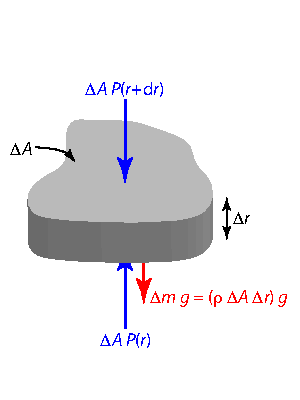
\includegraphics[width=\linewidth]{hydrostatic-equilibrium}
\caption[A fluid element in hydrostatic equilibrium]{A fluid element in hydrostatic equilibrium.
\label{f.hydrostatic-equilibrium}}
\end{marginfigure}

The force on the upper face is $\Delta A\times P(r+\Delta r)$; on the lower face, $\Delta A\times P(r)$.  Here $P(r)$ is the pressure.  For the element to be in hydrostatic equilibrium the forces must balance,
\[
        \Delta A \left[ -P(r+\Delta r) + P(r) - \Delta r \rho g(r)  \right] = 0;
\]
substituting for $g(r)$, dividing by $\Delta r$, taking the limit $\Delta r \to 0$ gives us the equation of hydrostatic equilibrium:
\begin{equation}\label{e.hydrostatic-equilibrium}
        \DD{P}{r} = -\rho \frac{Gm(r)}{r^{2}}.
\end{equation}
Here the mass enclosed within radius $r$ is
\begin{equation}\label{e.mass-continuity}
	m(r) = 4\pi \int_{0}^{r}\rho(r)r^{2}\,\dif r,
\end{equation}
with $\rho$ being the mass density. We can't solve these equations yet because we don't have a relation---yet---between $P$ and $\rho$.  But rather than wait to develop all of the physics we need, we are going to leapfrog ahead by \emph{assuming} a simple form for $\rho(r)$ and using that to understand better how stars work.

\begin{exercisebox}[A star of constant density]
\label{ex.constant-density-star}
Let's suppose that $\rho$ is constant throughout the star. 
In what follows, you should be able to express everything in terms of the star's mass $M$ and radius $R$, along with physical constants such as $G$ and $\kB$.

\begin{enumerate}
\item\label{rhoc} First, find $\rho$ in terms of the total mass $M$ and radius $R$.

\item Next, solve equation~(\ref{e.mass}) to find $m(r)$ in terms of $M$ and $r/R$.

\item\label{Pc} Use this expression for $m(r)$ and your expression for $\rho$ to integrate equation~(\ref{e.hydrostatic-equilibrium}) and to find the pressure at the center, $P_{c} = P(r=0)$.

\item
Now that we have an expression for the central pressure in terms of $M$ and $R$, let's try to understand what it means. For an ideal gas, the pressure, density, and temperature are related:
\begin{equation}\label{e.eos}
P = \rho\left(\frac{\kB}{\mu\mb}\right) T,
\end{equation}
where $\mb = 1/12\times(\textrm{mass of a \carbon\ atom})$ and $\mu$ is the mean molecular weight---the average mass of a particle in the gas.  We'll show how to compute $\mu$ later; for now, just treat it as a constant. Use your result from parts \ref{Pc} and \ref{rhoc}, as well as equation~(\ref{e.eos}) to find the central temperature of the star, in terms of $G$, $M$, $R$, and the mean molecular weight of the gas $\mu$.  Evaluate $T_{c}$ for $M=M_{\odot}$, $R=R_{\odot}$, and $\mu = 0.6$.  Do you get a reasonable result?
\end{enumerate}
\end{exercisebox}

With the assumption that $\rho = \textrm{constant}$, we showed (exercise~\ref{ex.constant-density-star}) that the central temperature and pressure depended on the total mass $M$, total radius $R$, and the gravitational constant $G$ as
\begin{eqnarray}
\label{e.Tc}
T_{c} &=& \frac{1}{2}\frac{GM}{R}\frac{\mu\mb}{\kB}\\
\label{e.Pc}
P_{c} &=& \frac{3}{8\pi}\frac{GM^{2}}{R^{4}}.
\end{eqnarray}
Here $\mu\mb$ is the average mass of a particle in the plasma. Our task now is to show that the scalings of $P$ and $T$ with $M$ and $R$ hold in general for an a star in mechanical equilibrium.

To show this, we are going to employ a form the \emph{virial theorem}.  Suppose we have a collection of $N$ particles, all moving about and exerting forces on one another.  If we let this system settle down into some kind of bound configuration, the virial theorem asserts that the kinetic energy $K$ is proportional to, and comparable in magnitude to, the potential energy $\Omega$; indeed if the potential between a pair of particles scales as $r^{-1}$, $r$ being the distance between the particles, then $K = -\Omega/2$.

Let us take the position and momentum of particle $i$ to be $\bvec{r}_{i} = (x_{i},y_{i},z_{i})$ and $\bvec{p}_{i}=(p_{x},p_{y},p_{z})$.  Then the total kinetic energy is
\begin{eqnarray}
\nonumber
	K &=& \frac{1}{2}\sum_{i=1}^{N}\bvec{p}_{i}\vdot\DDt{\bvec{r}_{i}}\\
		&=& \frac{1}{2}\left[\DDt{}\left(\sum_{i=1}^{N}\bvec{p}_{i}\vdot\bvec{r}_{i}\right) - \sum_{i=1}^{N}\bvec{r}_{i}\vdot\DDt{\bvec{p}_{i}}\right].
\label{e.expand-K}
\end{eqnarray}
The quantity $G = \sum_{i}\bvec{p}_{i}\vdot\bvec{r}_{i}$ is called the ``virial'' of the system.  By expressing the force $\bvec{F}_{i} = \dif\bvec{p}_{i}/\dif t$ on particle $i$ as the gradient of a potential $\Omega$, $\bvec{F}_{i} = -\grad_{i}\Omega$, we can rewrite eq.~(\ref{e.expand-K}) as
\begin{equation}\label{e.virial-deriv-1}
	2K = \DDt{G} + \sum_{i=1}^{N}\bvec{r}_{i}\vdot\grad_{i}\Omega.
\end{equation}
So far, we just shuffled and relabeled terms.  The crucial step comes in taking the time-average of the kinetic energy, which we'll denote by $\langle\;\rangle$:
\[	\langle f\,\rangle \equiv \lim_{\tau\to\infty} \frac{1}{\tau}\int_{0}^{\tau}f(t)\,\dif t. \]
Applying this to equation~(\ref{e.virial-deriv-1}) gives
\begin{eqnarray*}
	2\langle K\,\rangle &=&
		 \left\langle\DDt{G}\right\rangle 
		+ \left\langle\sum_{i=1}^{N}\bvec{r}_{i}\vdot\grad_{i}\Omega\right\rangle\\
	&=& \lim_{\tau\to\infty}\left[\int_{0}^{\tau}\,\DDt{G}\,\dif t\right] 
		+ \left\langle\sum_{i=1}^{N}\bvec{r}_{i}\vdot\grad_{i}\Omega\right\rangle\\
	&=& \underbrace{\lim_{\tau\to\infty}\left[\frac{G(\tau)-G(0)}{\tau}\right]}_{\mathrm{I}}
		+ \underbrace{\left\langle\sum_{i=1}^{N}\bvec{r}_{i}\vdot\grad_{i}\Omega\right\rangle}_{\mathrm{II}}
\end{eqnarray*}
Now, if the system is bound and in mechanical equilibrium, then the positions and momenta of all particles are finite: none of the particles can escape, and the system doesn't violently collapse so that momenta are diverging.  Hence both $G(\tau)$ and $G(0)$ are finite numbers, so as $\tau\to\infty$, term I vanishes.

As for term II, we can show that if the potential between pairs of particles depends on $1/r$, where $r$ is the distance between those particles, then term II is just $-\Omega$ (see Box~\ref{b.working-vectors}).  For now, I'll give a rough argument of why this is so:  in a spherically symmetric system, then the potential just depends on the distance $r$ from the origin; and since
\[
	r\dd{}{r} \left(\frac{1}{r}\right) = -\frac{1}{r},
\]
the last term is just $-\Omega$ and our equation is
\begin{equation}\label{e.virial-theorem}
2\langle K\,\rangle + \langle \Omega\rangle = 0.
\end{equation}
This is the virial theorem.

\begin{sidebar}[Working with vectors]
\label{b.working-vectors}
In this sidebar we'll show that the second term in equation~(\ref{e.virial-deriv-1}) is
\begin{equation}\label{e.term-2}
	\sum_{i=1}^{N}\bvec{r}_{i}\vdot\grad_{i}\Omega = -\Omega.
\end{equation}
First, we need an expression for $\Omega$. Suppose we pick a pair of particles, $i$ and $k$.  The potential between this pair is
\[
	-\frac{Gm_{i}m_{k}}{r_{ik}} = -\frac{Gm_{i}m_{k}}{\sqrt{(\bvec{r}_{i}-\bvec{r}_{k})^{2}}}.
\]
Our total potential consists of a sum over the potentials between all $N(N-1)/2$ unique pairs of particles,
\[
	\Omega = -\frac{Gm_{1}m_{2}}{\sqrt{(\bvec{r}_{1}-\bvec{r}_{2})^{2}}} - \ldots 
	-\frac{Gm_{i}m_{k}}{\sqrt{(\bvec{r}_{i}-\bvec{r}_{k})^{2}}} - \dots
\]
When we take the derivative in eq.~(\ref{e.term-2}), we apply $\bvec{r}_{i}\vdot\grad_{i}$ to each term in the potential.  For the term with the pair $i$, $k$, this will give
\begin{eqnarray*}
	\lefteqn{\sum_{i=1}^{N}\bvec{r}_{i}\vdot\grad_{i}\left(-\frac{Gm_{i}m_{k}}{\sqrt{(\bvec{r}_{i}-\bvec{r}_{k})^{2}}}\right)} \\
	&=& -Gm_{i}m_{k}\left[\bvec{r}_{i}\vdot\grad_{i}\left(\frac{1}{\sqrt{(\bvec{r}_{i}-\bvec{r}_{k})^{2}}}\right) + \bvec{r}_{k}\vdot\grad_{k}\left(\frac{1}{\sqrt{(\bvec{r}_{i}-\bvec{r}_{k})^{2}}}\right)\right].
\end{eqnarray*}
Since many of you aren't yet comfortable with vector expressions, we'll do this in detail for the $x$-component:
\begin{eqnarray*}
	\lefteqn{\left[\bvec{r}_{i}\vdot\grad_{i}\left(\frac{1}{\sqrt{(\bvec{r}_{i}-\bvec{r}_{k})^{2}}}\right) + \bvec{r}_{k}\vdot\grad_{k}\left(\frac{1}{\sqrt{(\bvec{r}_{i}-\bvec{r}_{k})^{2}}}\right)\right]_{x}}\\
	&=& x_{i}\dd{}{x_{i}}\left(\frac{1}{\sqrt{(\bvec{r}_{i}-\bvec{r}_{k})^{2}}}\right)
		+ x_{k}\dd{}{x_{k}}\left(\frac{1}{\sqrt{(\bvec{r}_{i}-\bvec{r}_{k})^{2}}}\right) \\
		&=& -\frac{x_{i}(x_{i}-x_{k})}{(\bvec{r}_{i}-\bvec{r}_{k})^{3/2}}
		+ \frac{x_{k}(x_{i}-x_{k})}{(\bvec{r}_{i}-\bvec{r}_{k})^{3/2}}\\
		&=& -\frac{(x_{i}-x_{k})^{2}}{(\bvec{r}_{i}-\bvec{r}_{k})^{3/2}}
\end{eqnarray*}
The $y$- and $z$-components are similar, giving
\begin{eqnarray*}
	\sum_{i=1}^{N}\bvec{r}_{i}\vdot\grad_{i}\left(-\frac{Gm_{i}m_{k}}{\sqrt{(\bvec{r}_{i}-\bvec{r}_{k})^{2}}}\right) &=& Gm_{i}m_{k}
	\frac{(\bvec{r}_{i}-\bvec{r}_{k})^{2}}{(\bvec{r}_{i}-\bvec{r}_{k})^{3/2}}\\
 &=& -\left(-\frac{Gm_{i}m_{k}}{\sqrt{(\bvec{r}_{i}-\bvec{r}_{k})^{2}}}\right).
\end{eqnarray*}
This can be done for every term in the sum, with the final result that
\[
	\sum_{i=1}^{N}\bvec{r}_{i}\vdot\grad_{i}\Omega = -\Omega.
\]
\end{sidebar}

For an ideal monatomic gas in thermal equilibrium, the mean kinetic energy of a particle in the gas is $K = (3/2)\kB T$, and we therefore may define an average temperature
\begin{equation}\label{e.Tbar}
	2 K = 3 N\kB \bar{T} = -\Omega.
\end{equation}
The total number of particles is $N=M/(\mu\mb)$, and so
\begin{equation}\label{e.mean-T}
\bar{T} = -\frac{1}{3}\Omega\frac{\mu\mb}{M\kB}.
\end{equation}
The total potential of the system depends on only three parameters: $G$, $M$, and $R$.  The only way to make a quantity having dimensions of energy is for
\[ \Omega \propto -\frac{GM^{2}}{R}, \]
and so
\[ \bar{T} \propto \frac{GM}{R}\frac{\mu\mb}{\kB}.  \]
By using the ideal gas law, $\bar{P} = \bar{\rho}(\kB/\mu\mb)\bar{T}$, we find
\[ \bar{P} \propto \frac{GM^{2}}{R^{4}}. \]
As a concrete example, let's compute $\Omega$ for a constant density sphere.
If we bring a small amount of mass $\dif m$ from infinity onto a sphere of mass $m$ and radius $r$, then the change in potential is \[ \dif\Omega = -\frac{Gm}{r}\,\dif m. \]
For a constant density, $r = R(m/M)^{1/3}$; upon substituting for $r$ we have
\[
	\Omega_{\textrm{const.\ den.}} = - \int_{0}^{M}\frac{GM^{1/3} m^{2/3}}{R}\,\dif m = -\frac{3}{5}\frac{GM^{2}}{R}.
\]
Using this in equation~(\ref{e.mean-T}) gives us the mean temperature, and hence pressure, for a constant density sphere,
\begin{eqnarray}\label{e.mean-T-rho}
\bar{T} &=& \frac{1}{5}\frac{GM}{R}\frac{\mu\mb}{\kB},\\
\label{e.mean-P}
\bar{P} &=& \frac{3}{20\pi}\frac{GM^{2}}{R^{4}}.
\end{eqnarray}
These are comparable to the central values, eqn.~(\ref{e.Tc}) and (\ref{e.Pc}).

\section{A closer look at hydrostatic equilibrium}
\label{s.closer-look}

Let's imagine what would happen if the star fell out of equilibrium.  Suppose we could turn off the pressure.  The star would collapse; how long would this take?  Let's calculate the amount of time a particle would need to free-fall from the surface to the center.  We can get this from Kepler's law. Start with a circular orbit and deform it while keeping the center at one focus, as shown in Fig.~\ref{f.fall-to-center}.  

The limit of these increasingly eccentric orbits is a fall into the center.  The time is one-half of an orbital period, and the semi-major axis in this limiting case is $a = R/2$:
\[
\tau_{\mathrm{ff}} = \frac{T}{2} = \frac{\pi}{\sqrt{GM}} \left(\frac{R}{2}\right)^{3/2}.
\]
Notice that we again have the combination $\sqrt{R^{3}/M}$.  Let's convert this into an expression involving the mean density $\bar{\rho}$:
\begin{equation}\label{e.tff}
\tau_{\mathrm{ff}} = \left(\frac{3}{32\pi}\right)^{1/2}\left(\frac{1}{G}\frac{4\pi R^{3}}{3M}\right)^{1/2} = \left(\frac{3}{32\pi}\right)^{1/2} \frac{1}{\sqrt{G\bar{\rho}}}.
\end{equation}
The time to collapse is proportional to $1/\sqrt{G\bar{\rho}}$ and depends on the average density of the star. We call $t_{\mathrm{dyn}} \equiv 1/\sqrt{G\bar{\rho}}$ the \emph{dynamical timescale} of the star.

\begin{marginfigure}[-12\baselineskip]
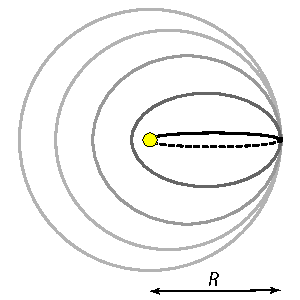
\includegraphics[width=\linewidth]{fall-to-center}
\caption[Fall to center]{\label{f.fall-to-center} Deformation of an orbit until it becomes a fall to the center, denoted by the yellow dot.}
\end{marginfigure}

Let's avoid a collapse by turning the pressure back on.  If part of the star is falling inward, the gas within the star will be compressed, the pressure will rise, and hydrostatic equilibrium will be restored.  How quickly can the star respond? A change is pressure is communicated to the rest of the star by sound waves, which travel at a speed (see Box~\ref{b.sound-speed})
\begin{equation}\label{e.speed-of-sound}
c_{s} = \left(\gamma\frac{P}{\rho}\right)^{1/2}
	= \left(\gamma\frac{\kB T}{\mu\mb}\right)^{1/2}.
\end{equation}
Here $\gamma$ is the adiabatic index: for an ideal monatomic gas, $\gamma = 5/3$.  How long would it take for a sound wave to go a distance $R$?  Using the expression for the average temperature of a constant density sphere from eq.~(\ref{e.mean-T-rho}), we find
\[
	\tau_{\mathrm{sc}} = \frac{R}{c_{s}} = R\left(\frac{3R}{GM}\right)^{1/2}
		= \left(\frac{3}{2\sqrt{\pi}}\right)\frac{1}{\sqrt{G\bar{\rho}}}.
\]
Both the sound-crossing time, $\tau_{\mathrm{sc}}$, and the free-fall time, $\tau_{\mathrm{ff}}$, are approximately equal to the dynamical timescale $1/\sqrt{G\bar{\rho}}$.  This is another way of looking at hydrostatic equilibrium: the star is able to remain in balance because the time for pressure disturbances to propagate, $\tau_{\mathrm{sc}}$, is comparable to the time for large-scale motions of the fluid, $\tau_{\mathrm{ff}}$.

\begin{sidebar}[The sound speed]
\label{b.sound-speed}
Suppose we have a long tube filled with gas at pressure $P(x,t) = P_{0}$, density $\rho(x,t) = \rho_{0}$, and velocity $u(x,t) = U_{0} = 0$. We then tap on one end of the tube; this causes a disturbance to propagate down the tube. Let's look at a small mass of fluid, located between $x$ and $x+\Delta x$; if the cross-sectional area of the tube is $A$, then the mass in this small volume is $\rho A\,\Delta x$.

As a result of the disturbance, the pressure in the tube becomes $P(x,t) = P_{0}+\sigma P_{1}(x,t)$. In this expression, $\sigma$ is a bookkeeping parameter that we'll eventually set to unity. We will expand our equations and keep only terms that are linear in $\sigma$. The fluid will also acquire a velocity $u(x,t) = \sigma u_{1}(x,t)$. This compresses or rarifies the gas: $\rho(x,t) = \rho_{0} + \sigma\rho_{1}(x,t)$.  Because the pressure in the tube is no longer uniform, our small mass will accelerate: 
\begin{eqnarray*}
	\rho A\,\Delta x \ddt{u} &=& A\,\Delta x\,(\rho_{0} + \sigma\rho_{1})\ddt{(0 + \sigma u_{1})}\\
	&\approx& \sigma\left[A\,\Delta x \rho_{0}\ddt{u_{1}}\right] + \mathcal{O}(\sigma^{2}).
\end{eqnarray*}
The corresponding force on our mass is
\[
	A \left[ P(x) - P(x+\Delta x) \right] \approx -\sigma A \left[P_{1}(x+\Delta x)-P_{1}(x)\right];
\]
equating this to the expression---to order $\sigma$---for the acceleration, taking the limit $\Delta x\to 0$, and canceling common factors gives
\begin{equation}\label{e.sound-speed-ut}
	\ddt{u_{1}} = -\frac{1}{\rho_{0}}\ddx{P_{1}}.
\end{equation}
Because of the non-uniform velocity, the volume and hence density of our little mass will also change:
\[
	\ddt{V} = A\left[u(x+\Delta x)-u(x)\right] 
		= \sigma A\,\Delta x\left[\frac{u_{1}(x+\Delta x)-u_{1}(x)}{\Delta x}\right]
\]
or
\begin{equation}\label{e.sound-speed-lnVt}
	\frac{1}{V}\ddt{V} = \sigma \ddx{u_{1}}.
\end{equation}
This change in volume is related to the change in pressure. We are interested in fluctuations that are sufficiently quick that no heat is transferred into or out of our mass. This is an adiabatic process, for which $PV^{\gamma} = \mathrm{const.}$. Here $\gamma$ is called the adiabatic index; for an ideal gas, this is the ratio of specific heats, $\gamma = C_{P}/C_{V}$.

As the pressure changes adiabatically from $P_{0}$ to $\sigma P_{1}$, the volume changes as
\[
	\frac{\dif V}{V} = \dif\ln V = -\frac{1}{\gamma}\dif\ln P.
\]
Hence
\begin{equation}\label{e.sound-speed-lnVt-2}
	\ddt{\ln V} = -\frac{1}{\gamma}\ddt{\ln (P_{0} + \sigma P_{1})} \approx 
		-\frac{\sigma}{\gamma P_{0}}\ddt{\ln P_{1}} = \sigma \ddx{u_{1}}.
\end{equation}
The last equality comes from equation (\ref{e.sound-speed-lnVt}).

We therefore have two equations for the perturbed velocity to order $\sigma$:
\begin{eqnarray*}
\ddt{u_{1}} &=& -\frac{1}{\rho_{0}} \ddx{P_{1}}\\
\ddx{u_{1}} &=& -\frac{1}{\gamma P_{0}} \ddt{P_{1}};
\end{eqnarray*}
differentiating the top equation with respect to $x$ and the bottom with respect to $t$, and equating the expressions for $\partial^{2}u_{1}/\partial t\partial x$ gives
\begin{equation}\label{e.sound-speed}
\frac{\partial^{2} P_{1}}{\partial t^{2}} = \left(\frac{\gamma P_{0}}{\rho_{0}}\right)
	\frac{\partial^{2} P_{1}}{\partial x^{2}}.
\end{equation}
This is the equation for a wave: the solutions are $P_{1}(x,t) = P_{1}(x\pm c_{s}t)$, where the sound speed is $c_{s} = \sqrt{\gamma P/\rho}$.
\end{sidebar}

For the sun, $\bar{\rho} = \val{1400}{\kilo\gram\usk\meter^{-3}} = \val{1.4}{\grampercc}$; this is just a bit denser than you.  The dynamical timescale for the sun is about one hour.

\begin{exercisebox}[Sound-crossing time]
The central temperature $T_{c}$ is a measure of the average kinetic energy of a particle at the stellar center. Use the central temperature that you found for the constant density star in exercise~\ref{ex.constant-density-star} and estimate the time that such a particle would take to cross a distance $R$. How does this time compare to the orbital period of a satellite orbiting just outside the stellar surface?
\end{exercisebox}

\section{Stellar Properties}
\label{s.stellar-properties}

We can infer a great deal from our simple virial scalings. Table~\ref{t.stellar-properties} provides masses and radii, in units of $\Msun$ and $\Rsun$, for stars from type B to type M.  If we assume that the stars have the same distribution of mass, so that the numerical coefficients in the expressions for $\rho_{c}$, $T_{c}$, and $P_{c}$ are the same, then for each star we may compute $\rho_{c}/\rho_{c,\odot} = (M/\Msun)(R/\Rsun)^{-3}$ and similarly for $T_{c}/T_{c,\odot}$ and $P_{c}/P_{c,\odot}$.

\begin{table}
\caption{\label{t.stellar-properties} Masses and radii for selected stellar types.}
\begin{tabular}{ld{4.2}d{3.2}d{1.2}d{1.2}d{1.2}d{2.3}}
 & \tabhead{B2} & \tabhead{B8} & \tabhead{F0} & \tabhead{G5} & \tabhead{M0} & \tabhead{M7}\\ 
\hline
$M/\Msun$ & 9.8 & 3.8 & 1.6 & 0.92 & 0.51 & 0.12\\
$R/\Rsun$ & 5.6 & 3.0 & 1.5 & 0.92 & 0.60 & 0.18\\
$L/\Lsun$ & 5800.0    & 180.0 & 6.5 & 0.79 & 0.08 & 0.003\\
$\rho_{c}/\rho_{c,\odot}$ & 0.06 & 0.14 & 0.47 & 1.18 & 2.36 & 20.58\\
\rowcolor{yellow}
$T_{c}/T_{c,\odot}$ & 1.75 & 1.27 & 1.07 & 1.00 & 0.85 & 0.67\\
$P_{c}/P_{c,\odot}$ & 0.10 & 0.18 & 0.51 & 1.18 & 2.01 & 13.72\\
\end{tabular}
\end{table}

Notice that $P_{c}$ and $\rho_{c}$ are larger for lower-mass stars. An even more surprising finding from this table is how little $T_{c}$ varies. This table spans nearly two decades in mass and six decades in luminosity, and yet $T_{c}$ varies by only a factor of three.  As we'll derive later, this is a consequence of the fusion reactions being extremely sensitive to temperature.

\section{Contraction to the main sequence}
\label{s.stellar-contraction}

Stars are born when a cold, dense\sidenote{Dense is a relative term; here we mean $\sim 100$ \emph{atoms} per cubic centimeter} cloud of gas and dust becomes unstable to gravitational collapse. The details of this process is a topic of current research; for our purposes, however, after a period of time a pre-main sequence star forms.  This object is in hydrostatic balance, but with a radius much larger than its main-sequence value.  As you know from the previous discussion, its central temperature will therefore be too low for fusion reactions to be important.  What happens to this object?

The pre-main sequence star is in hydrostatic balance, so it doesn't collapse. But the interior, and hence the surface, is warm, so it radiates energy.  The only source of energy is gravitational, so the pre-main sequence star \emph{must} contract.  How long would this take?  For our sun, the total energy is
\[
	E_{\odot} = K + \Omega = \Omega/2 \approx -\frac{G\Msun^{2}}{\Rsun};
\]
the time to radiate this energy away is
\begin{equation}\label{e.kelvin-helmholtz}
t_{\mathrm{KH}} = \frac{|E_{\odot}|}{\Lsun} \approx \frac{G\Msun^{2}}{\Rsun\Lsun} \approx \val{\sci{3}{7}}{\yr}.
\end{equation}
This timescale is called the \emph{Kelvin-Helmholtz timescale}.  Since $t_{\mathrm{KM}} \gg t_{\mathrm{dyn}}$ the star is, to an excellent approximation, in hydrostatic equilibrium throughout the whole contraction.

As the star contracts and $R$ decreases, the central density, pressure, and temperature increase.  When the central temperature becomes sufficiently hot, the heating from nuclear reactions rapidly increases and supplies enough energy to offset that radiated from the surface.  At this point the star is on the main-sequence, where it remains until the hydrogen fuel is exhausted from its core.

